\documentclass[12pt,twoside]{article}

\usepackage[english]{babel}
\usepackage[utf8]{inputenc}
\usepackage{sansmathfonts}
\usepackage[T1]{fontenc}
\renewcommand*\familydefault{\sfdefault} %% Only if the base font of the document is to be sans serif
\usepackage{multicol,lipsum}
\usepackage{amsmath,cancel}
\usepackage{amssymb,amsthm,dsfont,mathrsfs}
\usepackage[colorinlistoftodos]{todonotes}
\usepackage{geometry}
\geometry{
a4paper,
total={170mm,257mm},
left=20mm,
top=15mm,
bottom=22mm,
}
\usepackage{natbib}
\usepackage{soul}
\usepackage{setspace}
\usepackage{hyperref}
\usepackage{xcolor}
\usepackage{graphicx}
\usepackage{tikz}
\usepackage{siunitx}
\graphicspath{ {imagens/} }
\usepackage{fancyhdr}
\pagestyle{fancy}
\renewcommand{\headrulewidth}{0pt}

\color{darkgray}
\newcommand{\T}[1]{\vspace{0.4cm}\textbf{\large#1}}
\newcommand{\TW}[1]{\textbf{\large#1}}

\newcommand{\TM}[1]{\vspace{0.2cm} \textbf{#1}}

\newcommand{\M}[1]{
\vspace{-0.6cm}
\begin{flalign*}
#1&
\end{flalign*}
\vspace{-0.6cm}
}


\definecolor{bluebell}{rgb}{0.25, 0.35, 0.89} 
\definecolor{laranja}{rgb}{0.87, 0.48, 0.25} 
\definecolor{verde}{rgb}{0, 0.54, 0.44} 
\definecolor{babypink}{rgb}{1, 0.42, 0.52} 
\definecolor{rosa}{rgb}{1, 0.72, 0.77} 
\definecolor{cinza}{rgb}{0.3, 0.3, 0.3}  
\definecolor{iris}{rgb}{0.25, 0.35, 0.89}  
\definecolor{babyblue}{rgb}{0.13, 0.59, 0.95}

\setlength\columnsep{30pt}

\setlength{\parindent}{0cm}
\setlength{\fboxrule}{1.3pt}  % <-- Aumenta a espessura

\newcommand{\Formula}[1]{
\begin{center}
\color{iris}
\fcolorbox{rosa}{white}{
\(
\begin{array}{c}
#1
\end{array}
\)
}
\color{cinza}
\end{center}
}

\begin{document}
\pagenumbering{gobble}


\includegraphics[width=4cm]{Logo2.png}
\begin{center}
    \textbf{\Huge \textcolor{bluebell}{Plano Cartesiano}}
\end{center}
\vspace{0.5cm}

\begin{multicols}{2}

% ── EIXOS E ORIGEM ────────────────────────────────────────────────────────────
\TW{Eixos e Origem}

O \textbf{plano cartesiano} é formado por duas retas numéricas perpendiculares:

\textbf{Eixo $x$} (horizontal — abscissas): positivo à direita, negativo à esquerda.

\textbf{Eixo $y$} (vertical — ordenadas): positivo acima, negativo abaixo.

\textbf{Origem $O(0,0)$}: ponto de interseção dos eixos.

\begin{center}
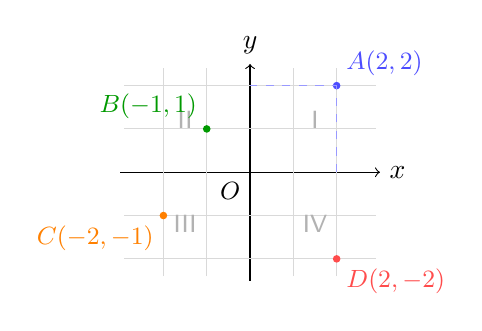
\begin{tikzpicture}[scale=0.55]
  \draw[->] (-3,0) -- (3,0) node[right] {$x$};
  \draw[->] (0,-2.5) -- (0,2.5) node[above] {$y$};
  % grid light
  \foreach \x in {-2,-1,1,2} \draw[gray!30] (\x,-2.4)--(\x,2.4);
  \foreach \y in {-2,-1,1,2} \draw[gray!30] (-2.9,\y)--(2.9,\y);
  % quadrant labels
  \node[gray!60, font=\small] at (1.5, 1.2)  {I};
  \node[gray!60, font=\small] at (-1.5,1.2)  {II};
  \node[gray!60, font=\small] at (-1.5,-1.2) {III};
  \node[gray!60, font=\small] at (1.5,-1.2)  {IV};
  % points
  \fill[blue!70]  (2,2)  circle (2.5pt) node[above right, font=\small] {$A(2,2)$};
  \fill[green!60!black] (-1,1) circle (2.5pt) node[above left, font=\small] {$B(-1,1)$};
  \fill[orange] (-2,-1) circle (2.5pt) node[below left, font=\small] {$C(-2,-1)$};
  \fill[red!70] (2,-2)  circle (2.5pt) node[below right, font=\small] {$D(2,-2)$};
  % projections A
  \draw[blue!40, dashed] (2,0)--(2,2)--(0,2);
  % origin
  \node[below left, font=\small] at (0,0) {$O$};
\end{tikzpicture}
\end{center}

\begin{center}
\small
\begin{tabular}{|c|c|c|}
\hline
\textbf{Quad.} & $x$ & $y$ \\ \hline
I   & $+$ & $+$ \\ \hline
II  & $-$ & $+$ \\ \hline
III & $-$ & $-$ \\ \hline
IV  & $+$ & $-$ \\ \hline
\end{tabular}
\end{center}

% ── LOCALIZAÇÃO DE PONTOS ─────────────────────────────────────────────────────
\TW{Localização de Pontos}

Cada ponto é um \textbf{par ordenado} $(x, y)$: a \emph{ordem importa},
$(2,3) \neq (3,2)$.

Para marcar $P(3,-1)$: mova 3 para a direita, depois 1 para baixo.

\TM{Em qual quadrante está $Q(-4, 2)$?}

$x < 0$ e $y > 0$ $\Rightarrow$ \textbf{Quadrante II}.

% ── DISTÂNCIA À ORIGEM ────────────────────────────────────────────────────────
\TW{Distância à Origem}

\Formula{d(P, O) = \sqrt{x^2 + y^2}}

Os catetos $|x|$ e $|y|$ formam um triângulo retângulo com $d$ como hipotenusa.

\TM{Exemplo 1 — $A(3,4)$}

$$d = \sqrt{9+16} = \sqrt{25} = \boxed{5}$$

\TM{Exemplo 2 — $B(-1,-1)$}

$$d = \sqrt{1+1} = \sqrt{2} \approx 1{,}41$$

% ── PARES SIMÉTRICOS ──────────────────────────────────────────────────────────
\TW{Pares Simétricos}

Dado $P(a, b)$:

\begin{tabular}{ll}
Eixo $x$: & $(a, -b)$ \\
Eixo $y$: & $(-a, b)$ \\
Origem: & $(-a, -b)$
\end{tabular}

\TM{Exemplo — $P(3, 2)$}

Eixo $x$: $(3,-2)$ \quad Eixo $y$: $(-3,2)$ \quad Origem: $(-3,-2)$

\fcolorbox{laranja}{white}{\parbox{0.85\linewidth}{
\small O simétrico à origem inverte os dois sinais — equivale a duas reflexões seguidas.
}}

\end{multicols}

\lfoot{\scriptsize © Copyright, Pratique Já}
\cfoot{\large \textcolor{bluebell}{pratiqueja.com}}
\end{document}
